\documentclass{article}%
\usepackage[T1]{fontenc}%
\usepackage[utf8]{inputenc}%
\usepackage{lmodern}%
\usepackage{textcomp}%
\usepackage{lastpage}%
\usepackage[head=40pt,margin=0.5in,bottom=0.6in]{geometry}%
\usepackage{graphicx}%
%
\title{\textbf{Lo que se ignoró al regular el precio de la carne}}%
\author{Adriana Fernández | @adrianakfv | afernandez@el{-}nacional.com}%
\date{04/10/2018}%
%
\begin{document}%
\normalsize%
\maketitle%
\textbf{URL: }%
http://www.el{-}nacional.com/noticias/economia/que{-}ignoro{-}regular{-}precio{-}carne\_254301\newline%
%
\textbf{Periodico: }%
EN, %
ID: %
254301, %
Seccion: %
Economía\newline%
%
\textbf{Palabras Claves: }%
Economía, Escasez, Inflación, Sociedad\newline%
%
\textbf{Derecho: }%
2.10%
, Otros Derechos: %
3.1%
, Sub Derechos: %
2.10.1, 3.1.1%
\newline%
%
\textbf{EP: }%
NO\newline%
\newline%
%
\textbf{\textit{Un productor agropecuario del estado Táchira asegura que vender el producto a 90 bolívares por kilo es insuficiente para cubrir los costos de producción}}%
\newline%
\newline%
%
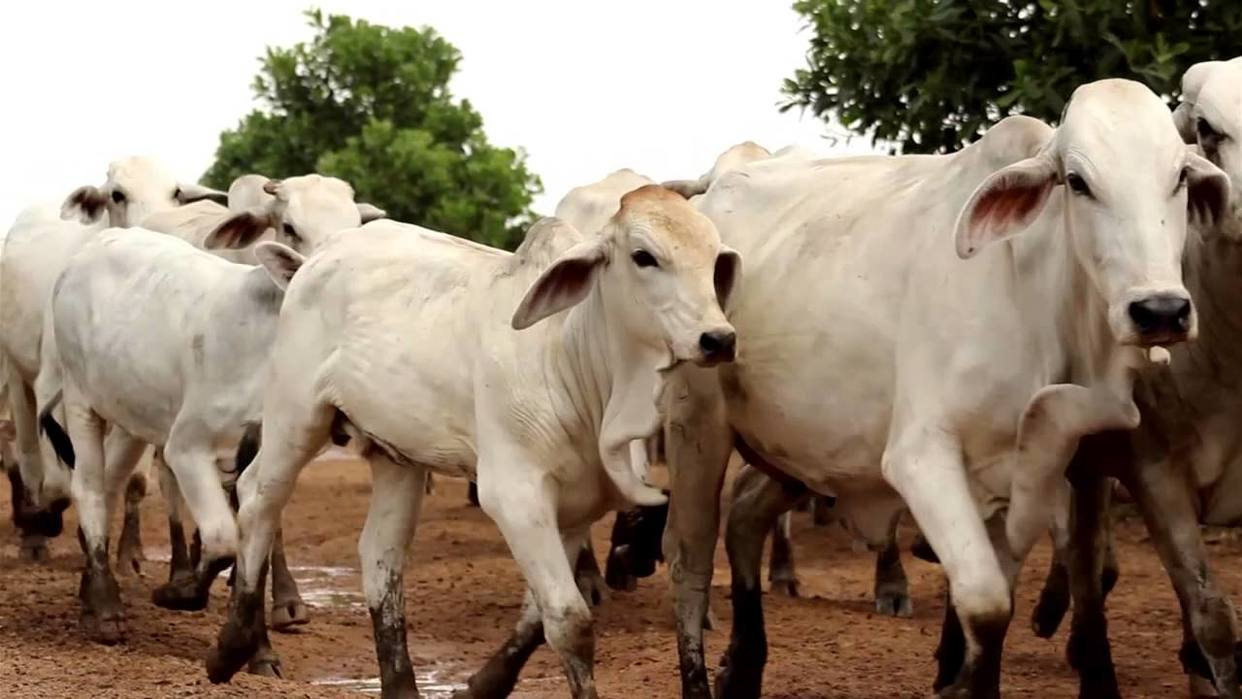
\includegraphics[width=300px]{1.jpg}%
\newline%
%
Luego de que el gobierno de Venezuela anunciara la regulación del precio de la carne a 90 bolívares por kilo, la producción del sector agropecuario del país ha desmejorado de forma considerable. Los ganaderos del estado Táchira, uno de los que genera la mayor cantidad de productos, han sido unos de los afectados por la medida económica implementada en agosto.%
\newline%
%
Heriberto Labrador, productor agropecuario de la entidad y economista, asegura que la cifra se basó únicamente en el precio final del producto, que dejó a un lado los costos de producción que los ganaderos deben cubrir para generar un litro de leche o un kilo de carne.%
\newline%
%
Señala que dicha situación ha provocado que los productores agropecuarios pierdan la capacidad para reponer los animales, por lo que se ha producido desabastecimiento en todo el territorio nacional.%
\newline%
%
“El tema no es generar abastecimiento simplemente, sino también generar reposición para que la cadena de comercialización no se rompa, es decir, que en el mediano y corto plazo siempre haya suministro. Si el ganadero no tiene capacidad de reponer lo que manda al matadero, en el corto plazo se va a generar un problema estructural, porque el desabastecimiento no va a ser por precio, sino por la falta de materia prima”, explicó Labrador.%
\newline%
%
Comentó que el precio de insumos como la medicina veterinaria y los rollos de alambre han tenido aumentos superiores al 120\%. “Eso no se está revisando, lo que se está revisando es simplemente el precio del producto a nivel del consumidor”, dijo.%
\newline%
%
Asegura que la ganadería es una labor que ha prevalecido en Táchira por al menos cuatro generaciones, por lo que los productores agropecuarios no especulan con el precio de la carne, el cual aseguran debe ser mucho mayor.%
\newline%
%
“Nadie nos va a venir a decir qué es lo que tenemos que hacer, eso lo sabemos hacer. Unos burócratas que están sentados en un escritorio desde Caracas no nos pueden imponer el precio final de un producto, porque no funciona así”, aseveró.%
\newline%
%
Escasez%
\newline%
%
La regulación de los precios no es el único problema que enfrentan los productores agropecuarios de Táchira. La falta de repuestos para maquinarias o equipos en el país los ha obligado en numerosas ocasiones a tener que trasladarse a Colombia para poder comprar los insumos.%
\newline%
%
La escasez de gasolina y diesel también se ha acentuado. Labrador comentó que los trabajadores deben emplear hasta cinco días para hacer una cola que les permita comprar el combustible, tanto para los vehículos de uso personal como para las maquinarias necesarias para el trabajo en las fincas.%
\newline%
%
Por otro lado, el aumento salarial decretado por el gobierno también generó un impacto negativo en el campo, debido a que la reducción de los ingresos por la regulación de los precios les impide a los dueños de las fincas cubrir la nómina de empleados que trabajan en ellas.%
\newline%
%
A pesar de ello, Labrador señala que tratan de brindarle a la mano obrera ciertas garantías para que siga trabajando en el sector agropecuario. “Tratamos de homologar los salarios a los de Colombia. Les damos los alimentos dentro de la finca para que el trabajador del campo tenga unas garantías mínimas que le permita seguir produciendo con nosotros”, acotó.%
\newline%
%
También destacó la disposición de los trabajadores a mantener su labor, a pesar de los obstáculos que representa desempeñar dicha actividad en Venezuela. Sin embargo, reconoce que el sector requiere de unas condiciones mínimas para poder trabajar.%
\newline%
%
“No se puede dejar de ser productor de la noche a la mañana, pero sí se puede dejar de ser eficiente, si no nos dan las condiciones para que podamos producir con tranquilidad y con algunas garantías mínimas”, dijo.%
\newline%
%
\end{document}